\documentclass{standalone}
\usepackage{tikz}
\usetikzlibrary{angles,quotes}
\begin{document}
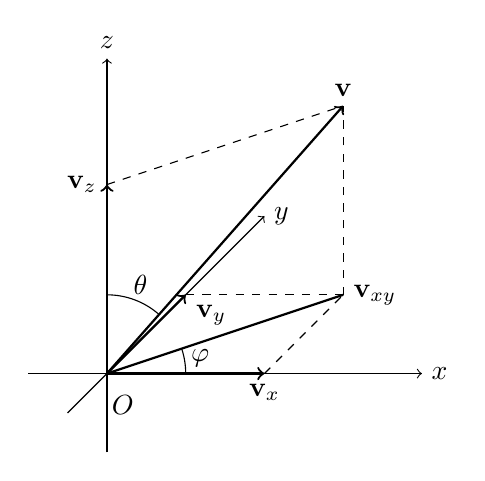
\begin{tikzpicture}[scale=2]
    \coordinate (O) at (0, 0);
    \node[black] at (0.1, -0.2) {$O$};
    \draw[->] (-0.5,0)--(2,0) coordinate (x) node[right]{$x$};
    \draw[->] (0,-0.5)--(0,2) node[above]{$z$};
    \draw[->] (-0.25, -0.25) -- (1, 1) node[right] {$y$};
    \draw[->, thick] (O) -- (1, 0) coordinate (vx) node[below] {$\mathbf{v}_x$};
    \draw[->, thick] (O) -- (0.5, 0.5) coordinate (vy) node[below right] {$\mathbf{v}_y$};
    \draw[dashed] (1,0) -- (1.5, 0.5);
    \draw[dashed] (0.5, 0.5) -- (1.5, 0.5);
    \draw[-, thick] (O) -- (1.5,0.5) coordinate (vxy) node[right] {$\mathbf{v}_{xy}$}; 
    \draw[->, thick] (O) -- (0, 1.2) coordinate (vz) node[left] {$\mathbf{v}_z$};
    \coordinate (O) at (0,0);
    \pic["$\varphi$", draw=black, -, angle eccentricity=1.2, angle radius=1cm] {angle=vx--O--vxy};
    \draw[dashed] (vxy) -- (1.5, 1.7) coordinate (v) node[above] {$\mathbf{v}$};
    \draw[dashed] (vz) -- (v);
    \draw[->, thick] (O) -- (v);
    \pic["$\theta$", draw=black, -, angle eccentricity=1.2, angle radius=1cm] {angle=v--O--vz};
\end{tikzpicture}
\end{document}